% Leroviditve
Az általunk tervezett rendszer architektúra diagramja a \ref{fig:architecture} ábrán látható. A rendszer frontend és backend része jól elkülöníthető egymástól, az egyes komponensek közötti kommunikáció titkosított HTTP kérések segítségével valósul meg. Először részletezzük a frontend és a backend felépítését, majd a közöttük megvalósuló kommunikációt.

\begin{figure}[H]
  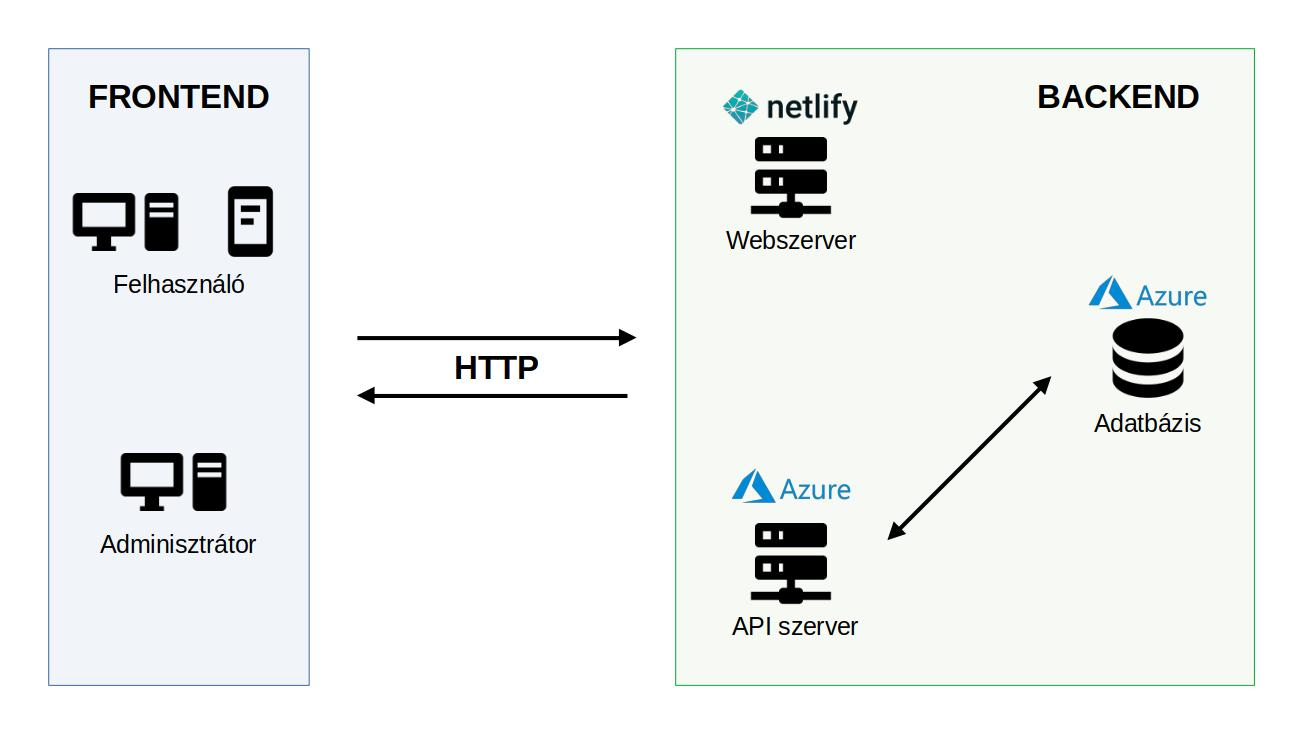
\includegraphics[width=\textwidth]{figures/architecture.jpg}
  \caption{A rendszer architektúrája}
  \label{fig:architecture}
\end{figure}

\section{Frontend}
A frontend a felhasználói felületet biztosítja, amelyen keresztül az emberek interakcióba léphetnek a rendszerrel. Jelen esetben a frontend két weboldalból és egy mobilalkalmazásból áll. A két weboldal teljesen elkülönül egymástól, mivel az egyik az adminisztrátoroknak, míg a másik a végfelhasználóknak készült. A weboldalak működése eltér a klasszikustól, mivel ezek egyoldalas alkalmazások (Single Page Application), így kliens oldali feldolgozást használnak, azaz a felhasználói felületet a kliens oldalon generálja a böngésző, nem pedig a webszerverről érkezik készen. Jelen esetben a webszerver csak a statikus fájlokat szolgáltatja, a dinamikus tartalmakat a kliens oldali JavaScript illeszti be az oldalakba. Ebből a szempontból a weboldal és a mobilalkalmazás működése megegyezik, mivel mindkettő direkt módon az API szerverrel kommunikál. Az adatok JSON típusú szövegként közlekednek a végpontok között az egyszerű feldolgozhatóság végett.

Fontos megemlíteni, hogy egyes API végpontokhoz azonosítás szükséges, ami úgynevezett JWT\footnote{JSON Web Token} tokonek segítségével valósul meg. Úgy a weboldalak, mint az alkalmazás eltárolják a szervertől kapott tokent és hozzáfűzik minden API kéréshez, ezzel azonosítva a felhasználót. Erre egy példa a \ref{fig:jwt} ábrán látható, ahol az adminisztrátorok számára megjelenített statisztikát kéri le a rendszer a backendtől. Ez a kérés egy Authorization fejléccel van ellátva, amely tartalmazza a JWT tokent.

\begin{figure}[H]
  \centering
  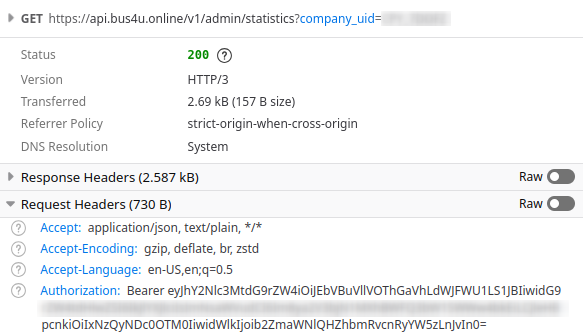
\includegraphics[width=0.7\textwidth]{figures/jwt.png}
  \caption{Azonosítást tartalmazó API kérés}
  \label{fig:jwt}
\end{figure}

Egyes oldalakon térképek is megjelennek, amelyeket a web esetében a MapBox, míg a mobil esetében a Google Maps szolgáltat. Mindkét esetben az adott platformhoz és technológiához közelebb álló térképszolgáltatót választottuk, hogy a lehető legjobb felhasználói élményt tudjuk biztosítani.

\section{Backend}
A backend a rendszer azon része, amely a kliens oldali felületek mögött fut, és biztosítja az adatok kezelését, tárolását, valamint az üzleti logika végrehajtását. A jelenlegi rendszerben a backend egy REST architektúrát követő API szerverként működik, amely Ruby on Rails technológiával készült. Ez az API szerver szolgálja ki mind a két weboldalt (adminisztrátori és végfelhasználói), valamint a mobilalkalmazást is.

A kliens oldali alkalmazások közvetlenül kommunikálnak a backend API végpontjaival, mindenféle köztes logika nélkül, így a rendszer architektúrája egyértelműen a kliens-szerver modellre épül.

A token alapú hitelesítést a rendszer a Devise felhasználókezelő könyvtár kiegészítéseként a devise-jwt gem segítségével valósítja meg. Ez lehetővé teszi a biztonságos, állapotmentes (stateless) autentikációt az API-n keresztül, anélkül hogy a szervernek külön munkameneteket (session-öket) kellene tárolnia.

A backend további feladatai közé tartozik az útvonalak, jegyek, bérletek, felhasználók, járművek és egyéb erőforrások adatainak kezelése, validálása és naprakészen tartása. A backend az adatokat egy PostgreSQL alapú relációs adatbázisban tárolja. Az adatok integritását és konzisztenciáját az ActiveRecord ORM réteg biztosítja, amely a Rails keretrendszer része.

A rendszer biztonsága érdekében az API végpontokhoz való hozzáférést szerepkör-alapú jogosultságkezeléssel szabályozzuk. Az adminisztrátorok számára elérhető végpontok például statisztikákat, jelentéseket és különféle menedzsment funkciókat biztosítanak, míg a végfelhasználók csak a saját jegyeikhez, bérleteikhez és a releváns útvonal-információkhoz férhetnek hozzá.

\section{Kommunikáció}
A felek közötti kommunikáció REST API hívásokkal valósul meg, ezt szemlélteti az \ref{fig:secvential-tickets} ábrán megjelenített szekvencia diagram, amely a felhasználó által megvásárolt jegyek listázásának folyamatát írja le. Amikor a felhasználó a frontend felületen keresztül a My Tickets oldalra navigál, egy GET kérés indul el a szerver felé, amely tartalmazza a felhasználó adatait. A backend először ellenőrzi a kérést, majd a megfelelő jegyeket lekérdezi az adatbázisból és visszaküldi a frontendnek, ahol azok idő szerinti rendezés után megjelennek a felhasználó számára. A még érvényes jegyekhez generál a rendszer egy QR kódot is, hogy könnyű legyen majd innen beolvasni. Amennyiben valahol hiba történik, a rendszer informálja erről a felhasználót. A következő kódrészlet intézi a kérést a frontend oldalról:

\begin{lstlisting}[language=JavaScript]
isLoading.value = true
axios.get('https://api.bus4u.online/v1/tickets_of_user', { headers: { Authorization: user.authorization }, params: { uid: user.uid }})
  .then(rsp => {
    isLoading.value = false
    tickets.value = rsp.data.sort((a, b) => {
      if(!a.is_valid && b.is_valid) return 1
      if(!b.is_valid && a.is_valid) return -1
      return b.date_of_purchase.localeCompare(a.date_of_purchase)
    })
    for(let i=0; i<tickets.value.length; i++) {
      if(!tickets.value[i].is_valid) continue
      QRCode.toDataURL(tickets.value[i].ticket_uid, { width: 250 }).then(rsp => tickets.value[i].qr = rsp)
    }
  }).catch(() => {
    tickets.value = []
    isLoading.value = false
  })
\end{lstlisting}

Egy ilyen kérésre, a backend által adott válasz az \ref{fig:response-tickets} ábrán látható.

\begin{figure}[H]
  \centering
  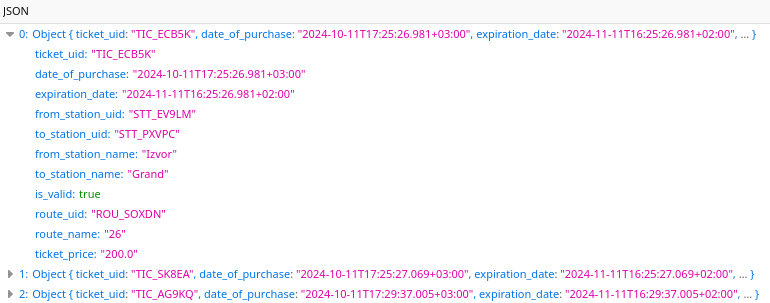
\includegraphics[width=0.9\textwidth]{figures/response-tickets.png}
  \caption{A jegyek listázásának válasza}
  \label{fig:response-tickets}
\end{figure}

\begin{figure}[H]
  \centering
  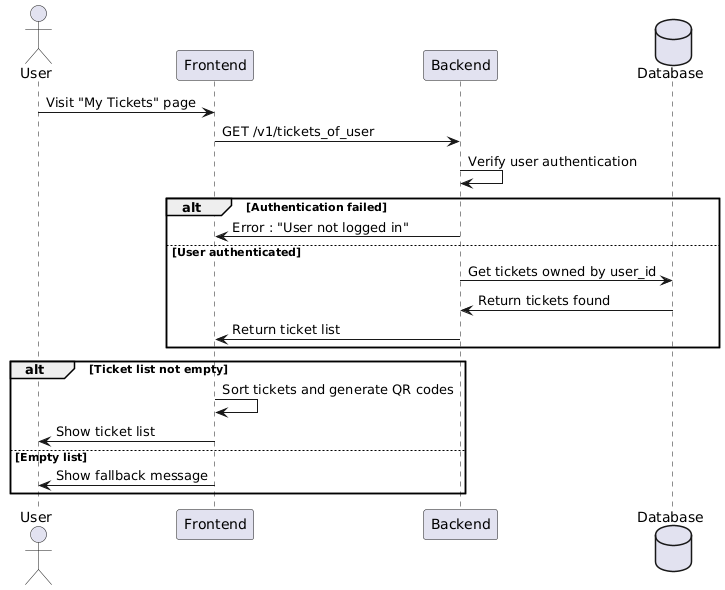
\includegraphics[width=0.9\textwidth]{figures/secvential-tickets.png}
  \caption{A jegyek listázásának folyamata}
  \label{fig:secvential-tickets}
\end{figure}

Ugyanígy leírható a regisztráció folyamata is, ahol a felhasználó megadja a nevét, az email címét és az új jelszót, majd a rendszer az adatok ellenőrzése után elküldi egyelőre csak az email címet a backend felé. A backend az email szerver segítségével küld egy 4 számjegyű kódot a felhasználó által megadott email címre. Ezután a felhasználó be kell írja ezt az ellenőrző kódot a felületen ennek megfelelő helyre. Ezt a kódot a backend ellenőrzi és amennyiben helyes, a frontend elküldi a felhasználó további adatait is, amelyet a backend elment az adatbázisban. Ha minden lépés sikeresen végrehajtódik, a frontend elmenti a bejelentkezési adatokat kliens oldalon is és átirányítja a felhasználót a főoldalra. Ellenkező esetben hibaüzenet jelenik meg a lépéssorozat azon pontján, ahol a hiba keletkezett. A regisztráció utolsó lépését (felhasználói adatok elküldése) megvalósító kódrészlet a következő:

\begin{lstlisting}[language=JavaScript]
async function sendForm() {
  axios.post('https://api.bus4u.online/auth', form).then((rsp) => {
    if(rsp.data.data.uid) {
      router.replace({ name: 'home' })
      user.signIn(rsp.data.data, rsp.headers)
    } else {
      isLoading.value = false;
    }
  }).catch((e) => {
    if(e.response) error.value = e.response.data.error;
    isLoading.value = false;
  });
}
\end{lstlisting}

\begin{figure}[H]
  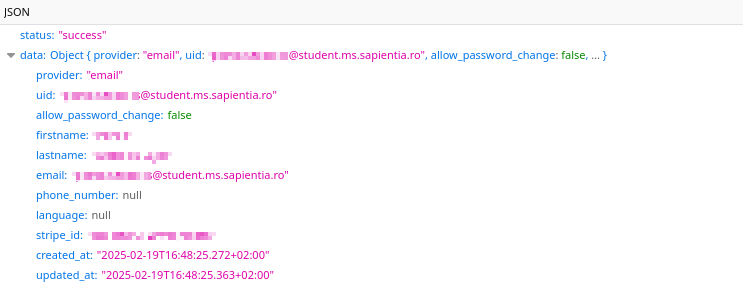
\includegraphics[width=\textwidth]{figures/response-registration.png}
  \caption{A regisztrációra adott válasz}
  \label{fig:response-registration}
\end{figure}

\newpage
A regisztrációs adatok elküldésére adott válasz az \ref{fig:response-registration} ábrán látható, míg a teljes regisztrációs folyamatot szemléltető szekvencia diagram az \ref{fig:secvential-registration} ábrán látható.

\begin{figure}[H]
  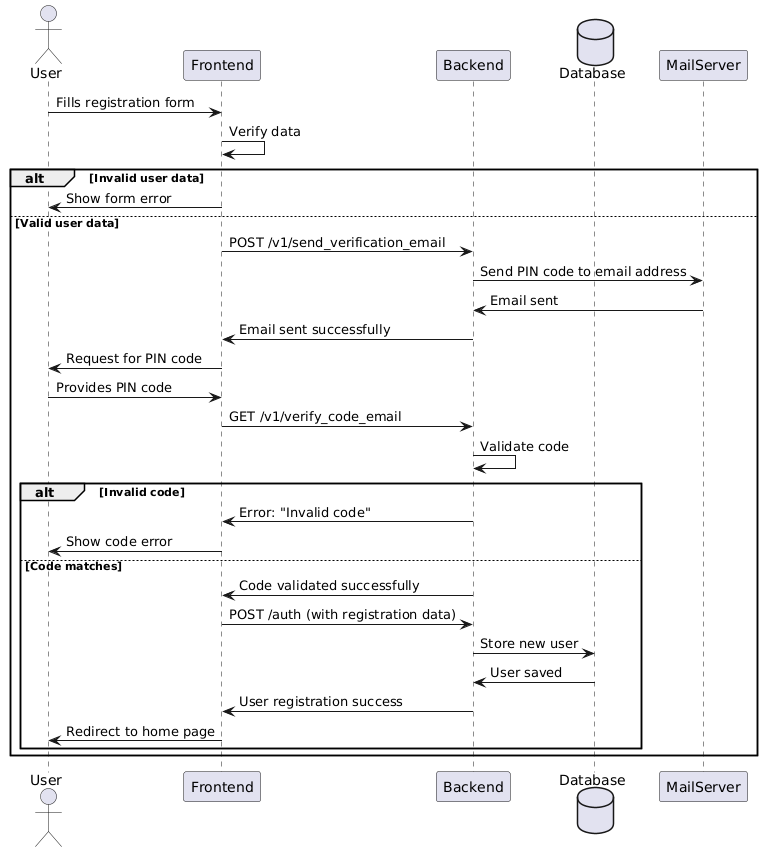
\includegraphics[width=\textwidth]{figures/secvential-registration.png}
  \caption{A regisztráció teljes folyamata}
  \label{fig:secvential-registration}
\end{figure}

\section{Felhasznált technológiák}

\subsection{Frontend}
A felhasználói és az admin weboldalak Vue.js keretrendszerben készültek, Vuetify komponenseket felhasználva. Azért esett a választás erre a kombinációra, mert a Vue által gyors és hatékony weboldalakat lehet létrehozni, a Vuetify pedig tovább gyorsítja a fejlesztést előre elkészített, jól kinéző komponensek szolgáltatásával.
A mobilra szánt alkalmazás elkészítéséhez Flutter technológiát használtunk, mert ennek segítségével egyetlen kódbázisból ki lehet generálni Android és iOS készülékekre is az alkalmazást, amely hatékonyan működik minden eszközön a keretrendszer optimalizációi miatt.

\subsubsection{Vue.js és Vuetify}
A Vue.js egy progresszív JavaScript keretrendszer, amelyet azért hoztak létre, hogy a webes felhasználói felületek fejlesztése egyszerűbb és gyorsabb legyen. A Vue.js abban különbözik a többi JavaScript keretrendszertől, hogy egy könnyű, gyors és hatékony technológiát kínál, amely egy Virtuális DOM modell segítségével gyorsítja a futást és amelynek a forráskódja akár 24 Kb-ra is zsugorítható, így viszonylag gyors a betöltése is \cite{vueinaction}.

A Vue.js két alapköve a deklaratív UI felépítés és a reaktivitás. Az első azt jelenti hogy az alap HTML kódot a Vue kiegészíti egy saját sablon-szintaxissal, amely lehetővé teszi a változók beékelődését a HTML kódba. A reaktivitás azt jelenti, hogy amikor a HTML sablonban felhasznált JavaScript változók értéke megváltozik, akkor a Vue érzékeli ezt és automatikusan megváltoztatja a megjelenített HTML kódot, így mindig a legfrissebb adatokat látja a felhasználó. Ugyanez végbemegy fordított irányban is, mert a felhasználói interakciók eredményeképpen a Vue automatikusan frissíti a háttérben lévő változókat is, így lesz a kommunikáció a DOM és a Vue között kétirányú \cite{vueinaction,vue3}.

A Vue keretrendszer egyik legnagyobb előnye, hogy könnyen tanulható és alkalmazható, így gyorsan lehet vele fejleszteni. Ennek egyik oka, hogy komponens alapú, amely lehetővé teszi a weboldalak felépítését újrafelhasználható, különálló komponensekből, amelyeket később össze lehet fűzni egy nagyobb alkalmazássá \cite{vue3}. Emellett a Vue nagyon jó online dokumentációval rendelkezik, amelyben minden funkció részletesen le van írva, de egyéb problémákkal és kérdésekkel a dinamikusan növekvő fejlesztői közösséghez is lehet fordulni \cite{vueinaction}.

A felhasználó szemszögéből a leglátványosabb tulajdonság, hogy nagyon gyors a navigáció, mivel a Vue Single Page Application üzemmódja által csak egyszer töltődik be a webalkalmazás, utána az oldalak közötti navigáció során csak a tartalom frissül, nem pedig az egész oldal, így kevesebb adat közlekedik a hálózaton és a böngészőnek is könnyebb dolga van a megjelenítésnél \cite{vue3}.

Fontos megemlíteni a Vue ökoszisztémájába tartozó egyéb eszközöket is, amelyek segítik a fejlesztést. Ilyen például a Vue Router, amely a weboldalak közötti navigációt teszi lehetővé, a Pinia, amely a globális állapotkezelést segíti, a Vite, amely a projekt generálását és a fejlesztést segíti \cite{vue3}. Léteznek UI könyvtárak is, például a Vuetify, amely lehetővé teszi a gyors és egyszerű felhasználói felületek készítését, azáltal hogy rengeteg előre elkészített, Material Design alapú Vue komponenst tartalmaz, amelyeket egyszerűen be lehet integrálni a weboldalba, így sok időt lehet vele spórolni. Az itt felsorolt technológiák segítségével gyorsan és hatékonyan sikerült felépíteni a weboldalak felhasználói felületeit, mi több, ezek jól néznek ki és jól is működnek minden tesztelt eszközön.

\subsubsection{Flutter}
A Flutter egy nyílt forráskódú, Google által kifejlesztett, cross-platform, UI készítő keretrendszer, amely lényege, hogy egyetlen kódbázisból ki lehet generálni az alkalmazásokat a legnépszerűbb platformokra. Ezek a platformok a következők: Android, iOS, Windows, macOS, Linux, valamint a web.

A Flutter a Dart programozási nyelvet használja, amely eredetileg a JavaScript lecserélésére volt létrehozva a webfejlesztésben, viszont idővel a Flutter technológia alapjává vált és így tett szert népszerűségre. A Flutter egyik nagy előnye, hogy egy widget rendszert használ, amely lehetővé teszi a felhasználói felületek egyszerű és gyors elkészítését. Ezek a widgetek alapértelmezetten a Material Designra épülnek, amely összhangban van a Vuetify webes komponenseivel is. A Flutter egy másik nagy előnye a hatékonyság, mivel natív kódra fordítja le a Dart kódot, így a lehető legjobb teljesítményt nyújtja, bármilyen platformról is legyen szó \cite{flutterinaction}.

Nagyban megkönnyíti a mobilra történő fejlesztést a Hot Reload, mivel a kódban történt változásokra azonnal reagál a felhasználói felület, így nem kell mindig újraindítani az alkalmazást \cite{flutterinaction}. A Flutterben való alkotás hatékonyságát tovább növeli, hogy részletes online dokumentációval rendelkezik, és hogy a Pub Package Manager-t (Csomagkezelőt) használja, amely rengeteg előre elkészített csomagot tartalmaz, az egyszerű UI komponensektől kezdve, a komplex háttérfolyamatokig.

\subsection{Backend}

A szerveroldali logika Ruby on Rails keretrendszer segítségével készült, amely lehetővé teszi a gyors fejlesztést és az átlátható, strukturált kódbázis kialakítását. A Rails erőssége, hogy számos beépített funkcióval rendelkezik, amelyek megkönnyítik az API-k létrehozását, az adatkezelést és a biztonságos működést. Az adatbázis kezelésére PostgreSQL-t választottunk, mivel megbízható, nyílt forráskódú relációs adatbázis-kezelő, amely jól skálázható és támogatja az összetett lekérdezéseket. A backend kiszolgálása az Azure felhőszolgáltatásban történik, amely rugalmasságot, automatikus skálázást és folyamatos rendelkezésre állást biztosít az alkalmazás számára.

\subsubsection{Ruby on Rails}
A Ruby on Rails egy népszerű és széles körben használt webes keretrendszer, amely a Ruby programozási nyelvre épül. A Rails két alapvető elv alapján működik: a „\textit{Convention over Configuration}” és a „\textit{Don’t Repeat Yourself}”. Ezek az elvek azt eredményezik, hogy a fejlesztőknek kevesebb kóddal kell dolgozniuk, mivel a Rails konvenciói automatikusan meghatározzák a konfigurációkat, így csökkentve a redundáns kódot és növelve a fejlesztési folyamat hatékonyságát \cite{hartl_rails, fernandez_rails}. Ez különösen hasznos nagyobb projektek esetén, mivel elősegíti a gyorsabb fejlesztést és az egyszerűbb karbantartást, amely a gyorsan változó üzleti igények mellett nélkülözhetetlen.

A Rails \textit{MVC (Model-View-Controller)} architektúrára épül, amely logikailag elkülöníti az alkalmazás különböző részeit: az adatkezelést (Model), a felhasználói felületet (View), és az üzleti logikát (Controller). Ez a struktúra átláthatóbbá teszi a kódot, mivel a különböző funkciók külön-külön karbantarthatók, anélkül hogy zavarnák egymást, valamint megkönnyíti az új funkciók hozzáadását is. A Rails alkalmazásokhoz számos „\textit{gem}”, vagyis könyvtár érhető el, amelyek előre elkészített megoldásokat kínálnak, így még a komplexebb funkciók integrálása is könnyebb és biztonságosabb lehet \cite{hartl_rails}.

A Rails további előnye, hogy natív módon támogatja \textit{RESTful API}-k létrehozását. A RESTful megközelítés egyértelmű, szabványosított formát biztosít az API-k számára, amely megkönnyíti az alkalmazások közötti integrációt, például egy mobilalkalmazás és a backend közötti kommunikáció során. Ennek a felépítésnek köszönhetően a Rails alkalmazások egyszerűen összekapcsolhatók más rendszerekkel és frontend megoldásokkal \cite{fernandez_rails}.

\subsubsection{PostgreSQL}
A PostgreSQL egy nyílt forráskódú, objektum-relációs adatbázis-kezelő rendszer, amely széles körben ismert teljesítményéről, rugalmasságáról, és különösen alkalmas komplex adatszerkezetek és nagy adattömegek kezelésére. Támogatja a fejlett adattípusokat, bonyolult lekérdezéseket, és párhuzamos műveleteket, amelyek különösen hasznosak a Bus4U-hoz hasonló, valós idejű adatokat feldolgozó rendszerekben \cite{douglas_postgresql, murrell_postgresql}.

A PostgreSQL kiválóan kezeli a párhuzamos lekérdezéseket és optimalizált módon képes kezelni nagy mennyiségű adatot és komplex lekérdezési struktúrákat. Ez biztosítja az alkalmazás gyors, megbízható működését, és lehetőséget nyújt az adatbázis hatékony méretezésére és finomhangolására az adatmennyiség növekedésével \cite{murrell_postgresql}.

Nagyobb adatmennyiség vagy felhasználói terhelés esetén a PostgreSQL támogatja a függőleges és vízszintes skálázást. Ezen túlmenően replikációval biztosítható a magas rendelkezésre állás, amely kritikus szempont a nagy terhelés alatt működő rendszerekben. Így a PostgreSQL hosszú távú, fenntartható teljesítményt és magas rendelkezésre állást biztosít, amely elengedhetetlen a Bus4U megbízható működéséhez \cite{douglas_postgresql}.

\subsubsection{Azure}
Az Azure egy olyan nagyvállalati szintű, biztonságos és skálázható felhőplatform, amely számos lehetőséget kínál modern alkalmazások fejlesztéséhez és működtetéséhez. Az Azure infrastruktúrája révén biztosítható a folyamatos és megbízható működés, míg a platform rugalmassága lehetővé teszi az erőforrások hatékony kezelését és a skálázhatóságot \cite{wilder_azure, collier_azure}. Az Azure használatával elkerülhetőek a hagyományos szerver infrastruktúrák fizikai korlátai, és olyan erőforrások válnak elérhetővé, amelyek az alkalmazás igényei szerint rugalmasan méretezhetők.

Az Azure automatikusan alkalmazkodik a változó terheléshez, amely lehetővé teszi, hogy a rendszer gördülékenyen kezelje a megnövekedett felhasználói forgalmat. Ez az adaptív megközelítés egy modern, folyamatosan növekedő alkalmazás számára elengedhetetlen, különösen tömegközlekedési rendszerek esetében, ahol a felhasználói igények időben változhatnak \cite{wilder_azure}.

Az Azure erőteljes adatvédelmi szabályokat és fejlett biztonsági protokollokat alkalmaz. Ezek közé tartozik a többfaktoros hitelesítés, a hálózati tűzfalak, valamint az adattitkosítás, amelyek biztosítják, hogy a Bus4U felhasználóinak adatai biztonságban legyenek. A platform megfelel a szigorú adatvédelmi szabványoknak, ami kulcsfontosságú egy olyan alkalmazás számára, amely szenzitív felhasználói adatokat kezel \cite{collier_azure}.


\section{Fejlesztői eszközök}

A fejlesztés során számos eszközt használtunk, amelyek segítették a a hatékonyságot. A legfontosabb ezek közül a kódszerkesztő, amelynek a Visual Studio Code-ot használtuk, mert ez egy könnyű, gyors és hatékony eszköz, amely jól testreszabható a rengeteg letölthető kiegészítő által, amelyeknek köszönhetően támogat szinte bármilyen programozási nyelvet és keretrendszert\footnote{Visual Studio Code: \url{https://code.visualstudio.com/}}.

Mivel a projekten ketten dolgoztunk, szükség volt egy eszközre amelyben vezetni tudjuk a feladatokat átlátható módon. Erre a Jira-t használtuk, amely egy online projektmenedzsment eszköz, amelynek segítségével könnyen lehet követni a feladatokat, a fejlesztés állapotát és a határidőket is egy kanban board-on.\footnote{A projekt Jira oldala: \url{https://bus4u.atlassian.net/jira}} Itt felbontottuk az egész projektet kisebb feladatokra, úgynevezett taszkokra, amelyekhez kódneveket rendeltünk hozzá. Ezeknek a formája \textit{BUS-XX} volt, ahol az \textit{XX} egy sorszám, amely a feladatok sorrendjét jelöli. A taszkok nevei tartalmazták a feladat rövid leírását, de hozzá lehetett adni bővebb leírást és hozzászólásokat is. A \ref{fig:jira} ábrán látható az általunk használt Jira tábla.

\begin{figure}[ht]
  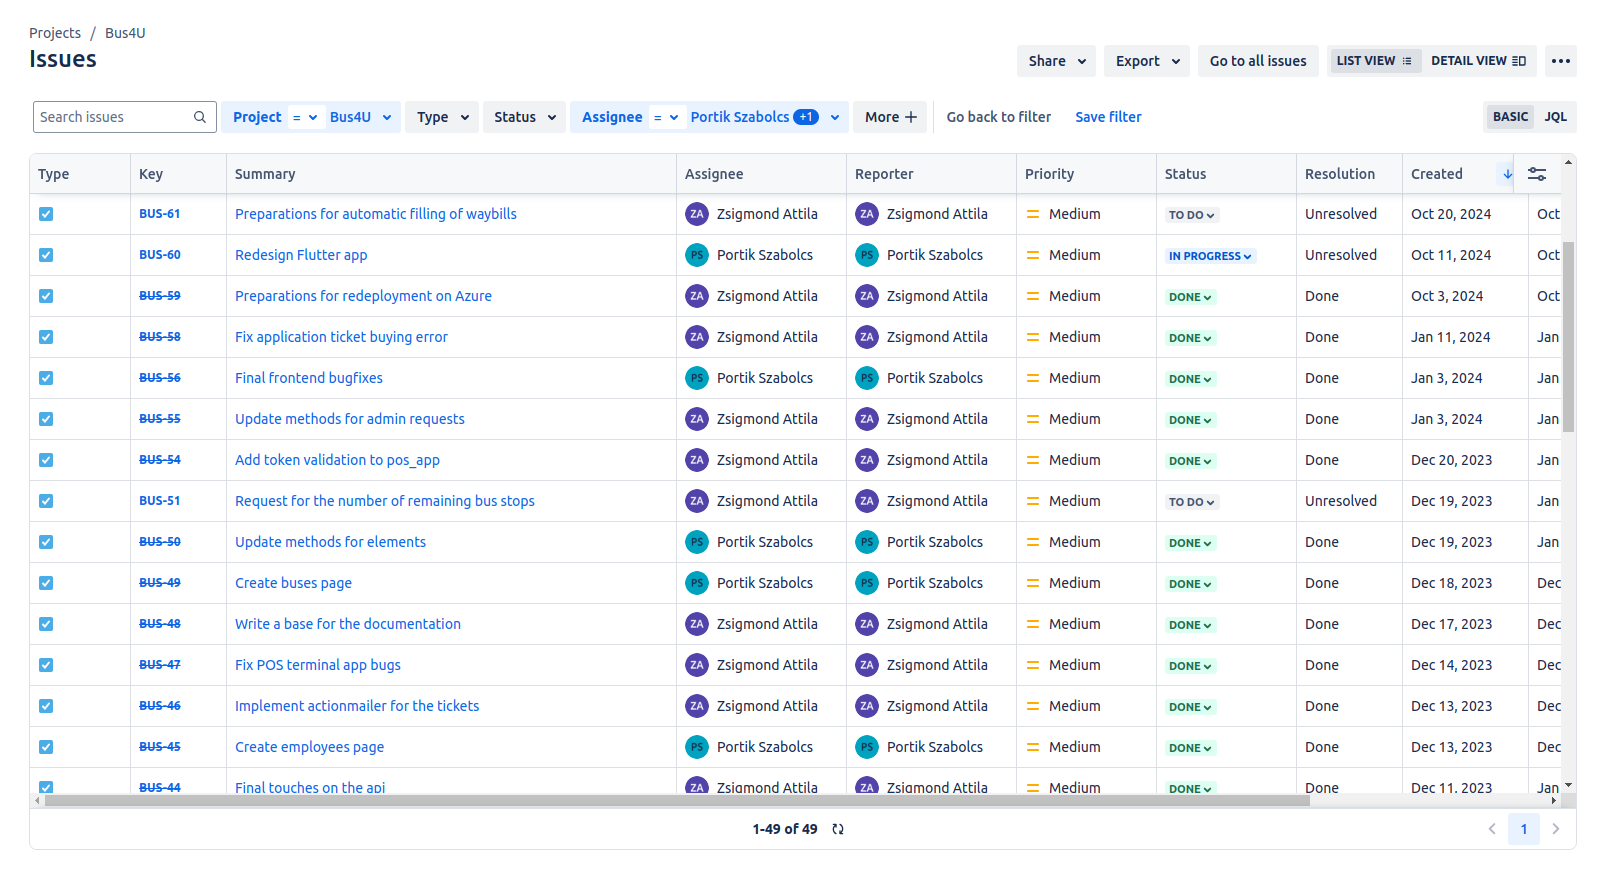
\includegraphics[width=\textwidth]{figures/jira.png}
  \caption{Feladatok a Jira-ban}
  \label{fig:jira}
\end{figure}

Verziókövetésre a Git-et használtuk, GitHub-al kiegészítve, így biztonságosan tudtuk tárolni a kódot és a változtatásokat is könnyen nyomon tudtuk követni. A GitHub abban is segített, hogy összehangoljuk a frontend és a backend fejlesztését, valamint hogy több, különböző eszközről is tudjunk dolgozni. A munka során branch-ekre (ágakra) osztottuk a projektet, úgy hogy a fő ág mellett volt egy develop nevű ág és ebből váltak ki az egyes feladatok mellékágai, amelyek mind egy-egy Jira taszknak feleltek meg. A mellékágak nevei tartalmazták a taszk kódját, így össze lehetett hangolni a verziókövetést a kanban táblával. A branchek használata megkönnyítette és strukturáltabbá tette a közös munkát.

\section{Kitelepítés}

\subsection{Azure infrastruktúra áttekintése}
A Bus4U rendszer a Microsoft Azure felhőalapú platformján került telepítésre. Az Azure szolgáltatások skálázhatóságot és megbízhatóságot biztosítanak a rendszer számára. A telepítéshez az alábbi főbb szolgáltatásokat használtuk:
\begin{itemize}
    \item Azure Virtual Machines (VM): A szerver hosztolása.
    \item Azure Database for PostgreSQL: Az adatbázis-szolgáltatás biztosítása.
\end{itemize}

\subsection{Domain konfiguráció}
A rendszer végpontjai az api.bus4u.online domainen érhetőek el, amelyet a Cloudflare platformján konfiguráltam. A domain hozzárendelése során a virtuális gép (VM) IP címét használtam. A következő beállításokat végeztem el:
\begin{itemize}
    \item DNS beállítások: A Cloudflare-en elvégeztem a domain névhez tartozó A és CNAME rekordok konfigurálását.
    \item SSL tanúsítványok: A HTTPS alapú kapcsolat biztonságának érdekében a Cloudflare szolgáltatásait alkalmazzuk, amelyek védelmet nyújtanak a felhasználók számára.
\end{itemize}


\subsection{Adatbázis telepítése és konfigurációja}
A rendszer adatbázisa egy Azure Database for PostgreSQL szolgáltatáson keresztül került telepítésre, amely lehetővé teszi az adatbázis automatikus méretezését és a folyamatos biztonsági mentések készítését. A következő beállításokat alkalmaztuk:
\begin{itemize}
    \item Titkosított kapcsolatok: A PostgreSQL adatbázis SSL tanúsítványokat használ a biztonságos kommunikációhoz.
    \item Backup és recovery: Automatikus biztonsági mentések kerülnek tárolásra az adatvesztés elkerülése érdekében.
\end{itemize}

\subsection{Szerver telepítése}
A szerver az Azure Virtual Machines szolgáltatásban került telepítésre, ahol a Ruby on Rails alapú API-t futtatjuk. A telepítés során a következő lépéseket hajtottuk végre:
\begin{itemize}
    \item Környezeti változók beállítása: A szükséges konfigurációs változók (pl. adatbázis kapcsolatok) a Ruby on Rails beépített credentials funkciójában lettek biztonságosan tárolva és kezelve.
    \item Verziókezelés: Az asdf verziókezelő használatával a Ruby és egyéb nyelvek verzióit könnyen kezelhetjük, ami megkönnyíti a fejlesztési környezet fenntartását.
    \item CI/CD pipeline: Az alkalmazás automatikus telepítése és frissítése a GitHub Actions integrációjával valósult meg.
\end{itemize}
A részletes telepítési folyamatot a \ref{fig:deployment-diagram} ábra szemlélteti.

\begin{figure}[H]
    \centering
    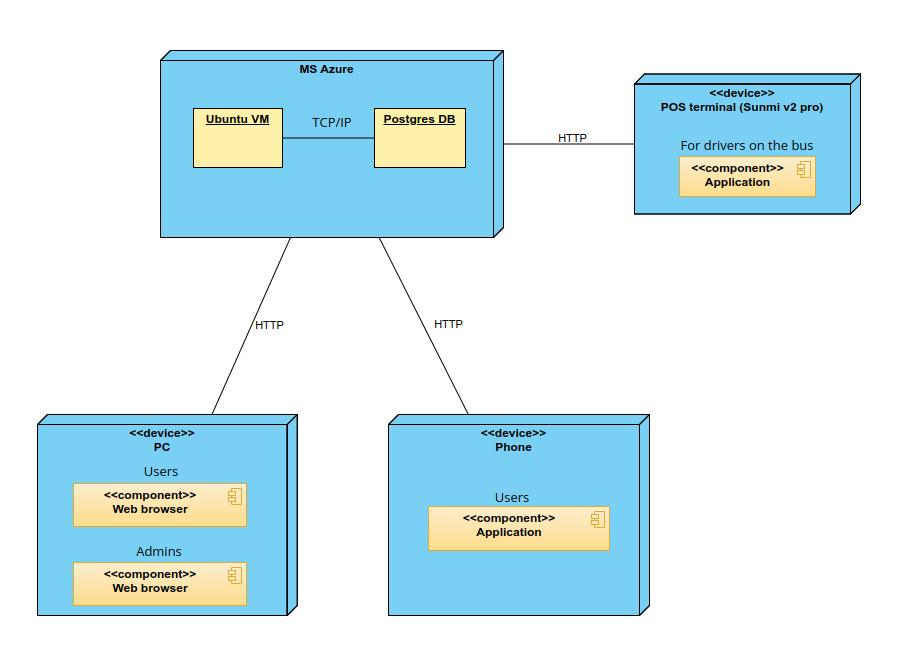
\includegraphics[width=\textwidth]{figures/deployment.jpg}
    \caption{Telepítési diagram}
    \label{fig:deployment-diagram}
  \end{figure}

A weboldalak ki lettek telepítve Netlify-ra, hogy könnyebben tesztelhetőek és bemutathatóak legyenek. A Netlify egy olyan szolgáltatás, amely lehetővé teszi a statikus weboldalak gyors és egyszerű kiszolgálását a GitHub repository-ból, így a változtatások a \textit{git push} parancs után azonnal megjelennek a weben. A felhasználói weboldal a \url{https://bus4u.online}, az adminisztrátori weboldal pedig a \url{https://admin.bus4u.online} címen érhető el.